% This is part of Mes notes de mathématique
% Copyright (c) 2006-2017
%   Laurent Claessens, Carlotta Donadello
% See the file fdl-1.3.txt for copying conditions.

%---------------------------------------------------------------------------------------------------------------------------
\subsection{Règles de calcul}
%---------------------------------------------------------------------------------------------------------------------------

\begin{proposition}[Règles de calculs]  \label{PROPooBWZFooTxKavX}
    Soient $f$ et $g$ des fonctions
  différentiables en $g(a)$ et $a$ respectivement, alors la composée
  $f\circ g$ est différentiable en $a$ et
  \begin{equation*}
    d (f\circ g)_a = d f_{g(a)} \circ d g_a
  \end{equation*}
  et de plus les jacobiennes correspondantes vérifient
  \begin{equation*}
      J_{f\circ g}(a) = J_f\big( g(a) \big)J_g(a)
  \end{equation*}
  où le membre de droite est le produit (non-commutatif !) des deux matrices.
\end{proposition}

\begin{corollary}[Chain rule] Si $f : \eR^p \to \eR$ et $g : \eR \to
  \eR^p$, alors
  \begin{equation*}
    (f\circ g)^\prime(t) = \sum_{i=1}^p \pder f {x_i}(g(t)) g_i^\prime(t).
  \end{equation*}
\end{corollary}

\begin{remark}
  \begin{enumerate}
  \item Si $p = 1$, on retrouve la règle usuelle de dérivation de
    fonctions composées.

  \item 
      Si $g$ est à plusieurs variables, cette règle permet de déterminer les dérivées partielles de $f \circ g$, puisqu'une dérivée partielle peut être vue comme dérivée usuelle par rapport à une seule variable (voir remarque page \pageref{deriveepartielles}).

  \item Si $f$ est à valeurs vectorielles, cette formule permet de
    retrouver la jacobienne de $f \circ g$ puisqu'il suffit de traiter
    chaque composante de $f$ séparément.
  \end{enumerate}
\end{remark}


\begin{definition}
	Une fonction $f:\eR^m\to \eR^n$ est dite \defe{différentiable sur l'ouvert $U\subset\eR^m$}{différentiable!sur un ouvert}, si $f$ est différentiable en tout point de $U$. Dans ce cas, la différentielle de $f$ est l'application
	\begin{equation}
		\begin{aligned}
			df\colon U\subset\eR^m&\to \aL(\eR^m,\eR^n) \\
			x&\mapsto df(x). 
		\end{aligned}
	\end{equation}
\end{definition}

\begin{remark}\label{rk_lin}
  Tout élément $T$ de $\mathcal{L}(\eR^m,\eR^n)$ est différentiable en tout point de $\eR^m$ et coïncide avec sa différentielle. En effet, pour tout $a$ et $h$ dans $\eR^m$  on a 
\[
\frac{\|T(a+h)-T(a)-T(h)\|_n}{\|h\|_m}=0.
\]
\end{remark}
La proposition \ref{diff1} nous donne une recette très pratique pour calculer la différentielle d'une fonction de $\eR^m$ dans $\eR^n$.

 \begin{definition}
	 Soit $f$ une fonction différentiable de $\eR^m$ dans $\eR$. On appelle \defe{gradient}{gradient} de $f$ la fonction $\nabla f : \eR^m\to \eR^m$\nomenclature{$\nabla f$}{gradient de la fonction $f$} de composantes
\[
\partial_{1}f,\ldots,\partial_{m}f. 
\] 
Soit $f$ une fonction de $\eR^m$ dans $\eR^n$, $f(a)=(f_1(a),\ldots,f_n(a))^T$. On appelle \defe{matrice jacobienne}{matrice!jacobienne} de $f$ la fonction $J(f) : \eR^m\to \eR^m\times\eR^n$ définie par
\begin{equation}
a\mapsto  \begin{pmatrix}
    \partial_{1}f_1(a) &\ldots&\partial_{m}f_1(a)\\
\vdots&\ddots&\vdots\\
\partial_{1}f_n (a)&\ldots&\partial_{m}f_n(a)\\
  \end{pmatrix}
\end{equation}
\end{definition}

%---------------------------------------------------------------------------------------------------------------------------
\subsection{Linéarité}
%---------------------------------------------------------------------------------------------------------------------------

La proposition suivante signifie que différentiation est une opération linéaire sur l'ensemble des fonctions différentiables. 
\begin{proposition}		\label{PropDiffLineaire}
  Soient $f$ et $g$ deux fonction de $U\subset\eR^m$ dans $\eR^n$ différentiables au point $a\in U$, et soit $\lambda$ dans $\eR$. Alors les fonctions $f+g$ et $\lambda f$ sont différentiables au point $a$ et on a 
  \begin{equation}
    \begin{aligned}
 &     d(f+g)(a)=df(a)+dg(a), \\
& d(\lambda f)(a)=\lambda df(a),
    \end{aligned}
\end{equation}
\end{proposition}
\begin{proof}
  \begin{equation}
    \begin{aligned}
     & \lim_{h\to 0_m}\frac{\left\|\left(f(a+h)+g(a+h)\right)-\left(f(a)+g(a)\right)-df(a).h-dg(a).h\right\|_n}{\|h\|_m}\leq\\
&\lim_{h\to 0_m}\frac{\|f(a+h)-f(a)-df(a).h\|_n}{\|h\|_m}+\lim_{h\to 0_m}\frac{\|g(a+h)-g(a)-dg(a).h\|_n}{\|h\|_m}=0.
    \end{aligned}
  \end{equation}
  De même on démontre la  propriété $d(\lambda f)(a)=\lambda df(a)$.
\end{proof}

%---------------------------------------------------------------------------------------------------------------------------
\subsection{Produit}
%---------------------------------------------------------------------------------------------------------------------------

Soient $f$ et $g$ deux fonctions de $\eR^m$ dans $\eR^n$. Nous notons $f\cdot g$ la fonction de $\eR^n$ dans $\eR$ donnée par le produit scalaire point par point, c'est à dire
\begin{equation}
	(f\cdot g)(x)=f(x)\cdot g(x)
\end{equation}
pour tout $x\in\eR^m$. Le point dans le membre de droite est le produit scalaire dans $\eR^n$. Le cas particulier $n=1$ revient au produit usuel de fonctions :
\begin{equation}
	(fg)(x)=f(x)g(x).
\end{equation}

\begin{lemma}		\label{LemDiffProsuid}
	Si $f$ et $g$ sont des fonctions différentiables sur $\eR^m$ à valeurs dans $\eR$, alors la fonction produit $fg$ est également différentiable et
	\begin{equation}		\label{EqDifffgProd}
		d(fg)(a)=df(a)g(a)+f(a)dg(a)
	\end{equation}
	au sens où pour chaque $u$ dans $\eR^m$,
	\begin{equation}
		d(fg)(a).u=g(a)df(a).u+f(a)dg(a).u.
	\end{equation}
\end{lemma}
Remarquons qu'ici, $f(a)$ et $g(a)$ sont des réels, donc nous pouvons écrire $f(a)dg(a)$ aussi bien que $dg(a)f(a)$ sans ambigüités. 

\begin{proof}
	Ce que nous devons faire pour vérifier la formule \ref{EqDifffgProd}, c'est de vérifier le critère \eqref{EqCritereDefDiff} en remplaçant $f$ par $fg$ et $T(h)$ par $g(a)df(a).h+f(a)dg(a).h$.

	Ce que nous avons au numérateur est
	\begin{equation}
		\begin{aligned}[]
			\clubsuit&=(fg)(a+h)-(fg)(a)-g(a)df(a).h-f(a)dg(a).h\\
				&=f(a+h)g(a+h)-f(a)g(a)-g(a)df(a).h-f(a)dg(a).h.
		\end{aligned}
	\end{equation}
	Maintenant, nous allons faire apparaître $\big( f(a+h)-f(a)-df(a) \big)g(a+h)$ en ajoutant et soustrayant ce qu'il faut pour conserver $\clubsuit$ :
	\begin{equation}
		\begin{aligned}[]
			\clubsuit&=\big( f(a+h)-f(a)-df(a).h \big)g(a+h)\\
					&\quad +f(a)g(a+h)+g(a+h)df(a).h\\
					&\quad -f(a)g(a)-g(a)df(a).h-f(a)dg(a).h.
		\end{aligned}
	\end{equation}
	Nous mettons maintenant $f(a)$ et $fd(a).h$ en évidence là où c'est possible :
	\begin{equation}
		\begin{aligned}[]
			\clubsuit&=\big( f(a+h)-f(a)-df(a).h \big)g(a+h)\\
				&\quad+f(a)\big( g(a+h)-g(a)-dg(a).h \big)\\
				&\quad+\big( g(a+h)-g(a) \big)df(a).h.
		\end{aligned}
	\end{equation}
    Nous devons maintenant considérer la limite
	\begin{equation}
		\lim_{h\to 0}\frac{ \| \clubsuit \| }{ \| h \| }.
	\end{equation}
    Étant donné que $f$ et $g$ sont différentiables, les deux premiers termes sont nuls :
    \begin{equation}
        \begin{aligned}[]
            \lim_{h\to 0}\frac{ \big( f(a+h)-f(a)-df(a).h \big)}{\| h \|}g(a+h)=0\\
            \lim_{h\to 0} f(a)\frac{ \big( g(a+h)-g(a)-dg(a).h \big)}{\| h \|}=0.
        \end{aligned}
    \end{equation}
    En ce qui concerne le troisième terme, en utilisant la norme d'une application linéaire, nous avons
	\begin{equation}
		\lim_{h\to 0} \frac{ \| df(a).h \| }{ \| h \| }\leq\sup_{h\in\eR^m}\frac{ \| df(a).h \| }{ \| h \| }=\| df(a) \|,
	\end{equation}
    et par conséquent
    \begin{equation}
        \begin{aligned}[]
            0&\leq\lim_{h\to 0} \| g(a+h)-g(a) \|\frac{ \| df(a).h \|\| h \| }{ \| h \| }\\
            &\leq \lim_{h\to 0} \| g(a+h)-g(a) \|\| df(a) \|=0
        \end{aligned}
    \end{equation}
    parce que $g$ est continue (la limite du premier facteur est nulle tandis que la norme de $df(a)$ est un nombre constant). Nous avons donc bien prouvé que la formule \eqref{EqDifffgProd} est la différentielle de $fg$ au point $a$.
\end{proof}
Ce résultat se généralise pour des fonctions $f$ et $g$ de $\eR^m$ dans $\eR^n$.

\begin{proposition}
	Soient $f$ et $g$ deux fonction de $U\subset\eR^m$ dans $\eR^n$ différentiables au point $a\in U$. Alors la fonction $f\cdot g$ est différentiable  au point $a$ et on a 
	\begin{equation}
		g(f\cdot g)(a)=g(a)\cdot df(a)+f(a)\cdot dg(a)
	\end{equation}
	au sens où
	\begin{equation}		\label{Eqdfcdotgexpl}
		d(f\cdot g)_a(u)=g(a)\cdot\big( df_a(u) \big)+f(a)\cdot\big( dg_a(u) \big)
	\end{equation}
	pour tout $u\in\eR^m$.
\end{proposition}
Note : il faut être bien attentif en lisant la formule \eqref{Eqdfcdotgexpl}. Les points à l'intérieur des grandes parenthèses marquent l'application des différentielles sur $u$. Le contenu de ces parenthèses sont donc des éléments de $\eR^n$. Les points devant les parenthèses dénotent le produit scalaire dans $\eR^n$ ($f(a)$ et $dg_a(u)$ sont des éléments de $\eR^n$).

\begin{proof}
	La preuve du cas $n=1$ est déjà faite; c'est la formule \eqref{EqDifffgProd}. Pour le cas général $n\geq 2$, nous passons au composantes en nous rappelant que
	\begin{equation}
		(f\cdot g)(a)=\sum_{i=1}^nf_i(a)g_i(a)=\sum_{i=1}^n(f_ig_i)(a).
	\end{equation}
	En utilisant la linéarité de la différentiation, nous nous réduisons donc au cas des produits $f_ig_i$ qui sont des fonctions de $\eR^m$ dans $\eR$ :
	\begin{equation}
		\begin{aligned}[]
			d(f\cdot g)(a)&=d\left( \sum_{i=1}^n f_ig_i \right)(a)\\
			&=\sum_{i=1}^n\big( df_i(a)g_i(a)+f_i(a)dg_i(a) \big)\\
			&=g(a)\cdot df(a)+f(a)\cdot dg(a).
		\end{aligned}
	\end{equation}
	Ceci termine la preuve.
\end{proof}

%---------------------------------------------------------------------------------------------------------------------------
\subsection{Différentielle de fonction composée}
%---------------------------------------------------------------------------------------------------------------------------

La plus importante entre les règles de différentiation est la règle de différentiation d'une fonction composée (\emph{chain rule} dans les livres anglais et américains). Cette règle généralise la règle de dérivation pour fonctions de $\eR$ dans $\eR$. Il est utile d'introduire d'abord une formulation équivalente de la définition de différentielle
\begin{lemma}\label{Def_diff2}
  Soit $U$ un ouvert de $\eR^m$. La fonction $f: U\to\eR^n$ est différentiable au point $a$ dans $U$, si et seulement s'il existe une fonction $\sigma_f: U\times U\to \eR^n$ telle que
  \begin{subequations}		\label{SubEqsDiff2}
	  \begin{align}
  		\sigma_f(a,a)&=\lim_{x\to a} \sigma_f(a,x)=0\\
		 f(x)&=f(a)+T(x-a)+\sigma_f(a,x)\|x-a\|_m,   \label{def_diff2}
	  \end{align}
  \end{subequations}
pour une certaine application linéaire $T\in\mathcal{L}(\eR^m,\eR^n)$.
\end{lemma}
\begin{proof}
	Si les conditions \eqref{SubEqsDiff2} sont satisfaites alors $T$ est la différentielle de $f$ en $a$. En effet, dans ce cas nous avons
	\begin{equation}
		f(a+h)=f(a)+T(h)+\sigma_f(a,a+h)\| h \|,
	\end{equation}
	et la condition \eqref{EqCritereDefDiff} devient
	\begin{equation}
		\lim_{h\to 0} \frac{ \| \sigma_f(a,a+h) \|\| h \| }{ \| h \| }=\lim_{h\to 0} \| \sigma_f(a,a+h)\| =0
	\end{equation}
	
 
Si $f$ est différentiable au point $a$ il suffit de prendre $T=df(a)$ et 
\[
\sigma_f(a,x)=\frac{f(x)-f(a)-df(a).(x-a)}{\|x-a\|_m}.
\]
\end{proof}

\begin{remark}
	La fonction $\sigma_f(a,x)\| x-a \|_m$ est ce qui avait été appelle $\epsilon(h)$ sur la figure \ref{LabelFigDifferentielle}.
\end{remark}

\begin{proposition}		\label{PropDiffCompose}
Soient $U$ un ouvert de $\eR^m$ et $V$ un ouvert de $\eR^n$. Soient $f: U\to V$  et $g: V \to \eR^p$ deux fonctions différentiables respectivement au point $a$ dans $U$ et $b=f(a)$ dans $V$. Alors la fonction composée $g\circ f: U\to \eR^p $ est différentiable au point $a$ et
\begin{equation}	\label{EqDiffCompose}
    d(g\circ f)_a=dg_{f(a)}\circ df_a.
\end{equation}
\end{proposition}

Note : la formule \eqref{EqDiffCompose} est à comprendre de la façon suivante. Si $u\in\eR^m$, alors
\begin{equation}
    d(g\circ f)_a(u)=\underbrace{dg_{f(a)}}_{\in\aL(\eR^n,\eR^p)}\Big( \underbrace{df_a(u)}_{\in\eR^n} \Big)\in\eR^p.
\end{equation}

\begin{proof}
 En tenant compte du lemme \ref{Def_diff2} on peut écrire 
 \begin{subequations}
	 \begin{align}
		f(a+h)-f(a)&=df_a(h)+\sigma_f(a,a+h)\|h\|_m,	&&\forall h\in U-a,\\
		g(b+k)-g(b)&=dg_b(k)+\sigma_g(b,b+k)\|k\|_n,	&&\forall k\in V-b.
	 \end{align}
 \end{subequations}
On sait que $f(a)=b$ et que $f(a+h)$ est  un élément de $V$ et $f(a+h)=f(a)+k$ pour $k=df(a).h+\sigma_f(a,a+h)\|h\|_m$.  Par substitution dans la deuxième équation on obtient 
\begin{equation}
	\begin{aligned}
		g\big(f(a+h)\big)& - g\big(f(a)\big)\\ 
        &=dg_{f(a)}\Big(df_a(h)+\sigma_f(a,a+h)\|h\|_m\Big)\\
		&\quad+\sigma_g\left(f(a), f(a+h)\right)\left\| df_a(h)+\sigma_f(a,a+h)\|h\|_m\right \|_n\\
		&=g\circ f (a+h) - g\circ f (a)\\
        &= dg_{f(a)}\circ df_a(h) \\
        &\quad +\|h\|_m\Big[ dg_{f(a)}\sigma_f(a,a+h)\\
		&\quad+\sigma_g\left(f(a), f(a+h)\right)\big\| df_a\frac{h}{\|h\|_m}+\sigma_f(a,a+h)\big \|_n\Big],
	\end{aligned}
\end{equation}
donc
\begin{equation}
	(g\circ f) (a+h) - (g\circ f) (a) = dg_f(a)\circ df_a(h) + S(a,a+h) \|h\|_m
\end{equation}
où $S$ représente le contenu du dernier grand crochet. Il ne reste plus qu'à prouver que $S(a,a+h)$ est $o(\|h\|_m)$. En tenant compte du fait que $\sigma_f(a,a+h)$ et $\sigma_g\left(f(a), f(a+h)\right)$ sont $o (\|h\|_m)$,
\begin{equation}
  \begin{aligned}
      & \lim_{h\to 0_m} \frac{S(a,a+h)}{\|h\|_m}= \lim_{h\to 0_m}\frac{dg_{f(a)}\sigma_f(a,a+h)}{\|h\|_m}+ \\
& + \lim_{h\to 0_m}\frac{\sigma_g\left(f(a), f(a+h)\right)\left\| df_a\frac{h}{\|h\|_m}+\sigma_f(a,a+h)\right \|_n}{\|h\|_m} = 0.
  \end{aligned}
\end{equation}
\end{proof}

En appliquant la proposition précédente point par point, nous obtenons le résultat suivant.
\begin{proposition}
Soient $U$ un ouvert de $\eR^m$ et $V$ un ouvert de $\eR^n$. Soient $f: U\to V$  et $g: V \to \eR^p$ deux fonctions différentiables respectivement sur $U $ et sur $V$. Alors la fonction composée $g\circ f: U\to \eR^p $ est différentiable sur $U$.
\end{proposition}
La matrice jacobienne de $g\circ f$ au point $a$ est le produit matriciel des matrices jacobiennes de $f$ et de $f$. Plus précisément, nous avons
\begin{equation}
	J_{g\circ f}(a)=J_g\big( f(a) \big)J_f(a).
\end{equation}
Remarquez que nous considérons la matrice jacobienne de $g$ au point $f(a)$.

Dans la cas particulier où $m=1$ et $f$ est une fonction d'un intervalle $I$ dans $\eR^n$, dérivable au point $a$, on a que la fonction composée $g\circ f$ est dérivable au point $a$ si $g$ est différentiable et alors
\[
(g\circ f)'(a)= dg\left(f(a)\right).f'(a).
\]
En fait, pour les fonction d'une seule variable la dérivabilité coïncide avec la différentiabilité.

Nous avons aussi une formule importante pour la différentielle des formes bilinéaires.
  \begin{lemma}\label{bilin_diff}
    Toute application bilinéaire 
    \begin{equation}
	    \begin{aligned}
		    B\colon \eR^m\times\eR^n&\to \eR^p \\
		    B(a_1,a_2)&=a_1 \star a_2
	    \end{aligned}
    \end{equation}
    est différentiable en tout point $(a_1,a_2)$ de $\eR^m\times\eR^n$, et on a
\[
dB(a_1,a_2).(h_1,h_2)=h_1\star a_2 + a_1\star h_2.
\] 
  \end{lemma}
  \begin{proof}
    \begin{equation}
      \begin{aligned}
  & \frac{\|B(a_1+h_1,a_2+h_2)-B(a_1,a_2)-(h_1\star a_2 + a_1\star h_2)\|_p}{\|(h_1,h_2)\|_{\eR^m\times\eR^n}} = \\ 
&= \frac{\|(a_1+h_1)\star(a_2+h_2)-a_1\star a_2-(h_1\star a_2 + a_1\star h_2)\|_p}{\|(h_1,h_2)\|_{\eR^m\times\eR^n}}=\spadesuit
 \end{aligned}
    \end{equation}
on rajoute et on enlève la quantité $(a_1+h_1)\star a_2$ dans le numérateur, et on obtient  
   \begin{equation}
      \begin{aligned}
%&= \frac{\|(a_1+h_1)\star(a_2+h_2)-(a_1+h_1)\star a_2 +(a_1+h_1)\star a_2- a_1\star a_2-}{\|(h_1,h_2)\|_{\eR^m\times\eR^n}}\\
%&\hspace{7cm}\frac{-(h_1\star a_2 + a_1\star h_2)\|_p}{\quad}=\\
&\spadesuit= \frac{\|(a_1+h_1)\star h_2+h_1\star a_2-(h_1\star a_2 + a_1\star h_2)\|_p}{\|(h_1,h_2)\|_{\eR^m\times\eR^n}}=\\
&= \frac{\|h_1\star h_2\|_p}{\|(h_1,h_2)\|_{\eR^m\times\eR^n}}\leq C\frac{\|h_1\|_m\|h_2\|_n}{\|(h_1,h_2)\|_{\eR^m\times\eR^n}}\leq\\
&\leq C\frac{\|(h_1,h_2)\|^2_{\eR^m\times\eR^n}}{\|(h_1,h_2)\|_{\eR^m\times\eR^n}}= C\|(h_1,h_2)\|_{\eR^m\times\eR^n}.
      \end{aligned}
    \end{equation}
Si on prend la limite de cette expression pour $(h_1,h_2)\to (0_m,0_n)$ on obtient $0$, donc la preuve est complète. À noter, que dans l'avant-dernier passage on a utilisé la continuité des applications linéaires $\pr_m:\eR^m\times\eR^n\to \eR^m$ et $\pr_n: \eR^m\times\eR^n\to \eR^n$ qui à chaque point $(a_1,a_2)$ de $\eR^m\times\eR^n$ associent $a_1$ et $a_2$ respectivement.  
\end{proof}

\begin{proposition}     \label{PropEKLTooSvZjdW}
    Soit \( V\) et \( W\) deux espaces vectoriels et \( \varphi\colon V\to W\) un isomorphisme. Soit \( f\colon \eC\to V\) une application telle que \(\varphi\circ f\colon \eC\to W\) soit différentiable.

    Alors \( f\) est différentiable et \( df=\varphi^{-1}\circ d(\varphi\circ f)\).
\end{proposition}

\begin{proof}
    Si \( T\) est la différentielle de \( \varphi\circ f\) au point \( z\) nous avons
    \begin{equation}
        \lim_{\substack{h\to 0\\h\in \eC}}\frac{ (\varphi\circ f)(z+h)-(\varphi\circ f)(z)+T(h) }{ h }=0.
    \end{equation}
    En appliquant \( \varphi\) aux deux membres, et en permutant avec la limite (parce que \( \varphi\) est continue),
    \begin{equation}
        \varphi\lim_{h\to 0} \frac{ f(z+h)-f(z)+\varphi^{-1} T(h) }{ h }=0,
    \end{equation}
    ce qui signifie que \( f\) est différentiable et que \( df=\varphi^{-1}\circ T=\varphi^{-1}\circ d(\varphi\circ f)\).
\end{proof}
  
%--------------------------------------------------------------------------------------------------------------------------- 
  \subsection{Différentielle et dérivées partielles}
%---------------------------------------------------------------------------------------------------------------------------

\begin{proposition}		\label{Diff_totale}
 Soit $U$ un ouvert dans $\eR^m$ et $a$ un point dans $U$. Soit $f$ une application de $U$ dans $\eR^n$. Si toute les dérivée partielles de $f$ existent sur \( U\) et sont continues au point $a$ alors $f$ est différentiable au point $a$.
\end{proposition}
\begin{proof} 
 On se limite au cas $m=2$.  Pour rendre les calculs plus simples on utilise ici la norme $\|\cdot\|_\infty$ dans l'espace $\eR^2$, mais comme on a vu plus en haut, cela ne peut pas avoir des conséquences sur la différentiabilité de $f$. Si la différentielle de $f$ au point $a$ existe alors elle est définie par la formule
\[
    df_a(v)=\frac{ \partial f }{ \partial x }(a)v_1+\frac{ \partial f }{ \partial y }(a)v_2
\] 
pour tout $v$ dans $\eR^m$. 

On commence par prouver le résultat en supposant que les dérivées partielles de $f$ au point $a$ sont nulles. La différentiabilité de $f$ signifie que pour toute constante  $\varepsilon> 0$ il y a une constante $\delta>0$ telle que si $\|v\|_\infty\leq \delta $ alors 
\[
\frac{\|f(a_1+v_1, a_2+v_2)-f(a_1, a_2)\|_n}{\|v\|_\infty}\leq \varepsilon. 
\]   
On écrit alors 
\begin{equation}
  \begin{aligned}
   & \|f(a_1+v_1, a_2+v_2)-f(a_1, a_2)\|_n=\\
&=\|f(a_1+v_1, a_2+v_2)-f(a_1+v_1, a_2)+f(a_1+v_1, a_2)-f(a_1, a_2)\|_n\leq\\
&\leq \|f(a_1+v_1, a_2+v_2)-f(a_1+v_1, a_2)\|_n+\|f(a_1+v_1, a_2)-f(a_1, a_2)\|_n.
  \end{aligned}
\end{equation}
Comme la dérivée partielle $\partial_x f$ est  nulle au point $a$  on sait que  pour toute constante  $\varepsilon> 0$ il y a une constante $\delta_1>0$ telle que si $|v_1|\leq \delta_1 $ alors
\[
\|f(a_1+v_1, a_2)-f(a_1, a_2)\|_n\leq \varepsilon |v_1|.
\] 
Pour l'autre terme on a, par la proposition \ref{val_medio_1},
\begin{equation}
  \begin{aligned}
   & \|f(a_1+v_1, a_2+v_2)-f(a_1+v_1, a_2)\|_n\leq \\
&\leq \sup\{\|\partial_yf(x)\|_n\,\vert\, x\in S\}|v_2|.
  \end{aligned}
\end{equation}
où $S$ est le segment d'extrémités  $(a_1+v_1, a_2)$ et $ (a_1+v_1, a_2+v_2)$. Comme la  dérivée partielle $\partial_y f$ est continue et nulle au point $a$ on sait que  pour toute constante  $\varepsilon> 0$ il existe une constante $\delta_2>0$ telle que si $\|(u_1,u_2)\|_\infty\leq \delta_2 $ alors $\|\partial_yf(a_1+u_1,a_2+u_2)\|_n\leq \varepsilon$. Si on choisit $\delta = \min\{\delta_1,\,\delta_2\}$ le segment $S$ est contenu dans la boule de rayon $\delta$ centrée au point $a$ et on obtient
\[
 \|f(a_1+v_1, a_2+v_2)-f(a_1, a_2)\|_n\leq \varepsilon |v_1|+\varepsilon |v_2|\leq 2\varepsilon \|v\|_\infty.
\]
Cela prouve que \( f\) est différentiable en \( (a_1,a_2)\) et que la différentielle est nulle :
\begin{equation}
    df_{(a_1,a_2)}=0.
\end{equation}

Dans le cas général, où les dérivées partielles de $f$ au point $a$ ne sont pas spécialement nulles, on peut considérer la fonction\footnote{Vous verrez dans la discussion à propos de la fonction \eqref{EqCJVooJOuXdN} pourquoi cette fonction ne fonctionne pas dans le cas de la dimension infinie.}
\begin{equation}    \label{EqXHVooJeQKrB}    
    g(x,y)=f(x,y)-\partial_1 f(a)x-\partial_2 f(a)y,
\end{equation}
qui a dérivées partielles nulles au point $a$. La fonction $g$ est donc différentiables. La fonction $f$ est maintenant la somme de $g$ et de la fonction linéaire et continue $(x,y)\mapsto \partial_1 f(a)x-\partial_2 f(a)y$. On verra dans la prochaine section que la somme de deux fonctions différentiables est une fonction différentiable. Par conséquent, la fonction $f$ est différentiable.
\end{proof}

\begin{remark}
    En dimension infinie, il n'est pas vrai que l'existence et la continuité de toutes les dérivées partielles en un point implique la différentiabilité en ce point. Pour donner un exemple, nous allons continuer l'exemple \ref{ExHKsIelG}
    avec la fonction \ref{EqCJVooJOuXdN} sur un espace de Hilbert.

    En dimension infinie nous aurons le théorème \ref{ThoOYwdeVt} qui donnera quelque chose de moins fort.
\end{remark}

Étant donné que pour tout vecteur $u$ dans $\eR^m$ on a $\partial_uf(a)=\nabla f(a)\cdot u$, le gradient de $f$ nous donne la direction dans laquelle la croissance de $f$ est maximale. Soit $C$ une colline et soit $f$ la fonction que a chaque point $(x,y)$ de la Terre associe son altitude. Si nous voulons monter la colline le plus vite possible nous n'avons qu'a suivre la direction $\nabla f$ à chaque point. Elle est la projection sur le plan $x$-$y$ de la direction de pente maximale. Au contraire, la direction $-\nabla f$ est la direction de croissance minimale.
   
La matrice jacobienne calculé au point $a$ est la matrice associée canoniquement à l'application linéaire $df_a:\eR^m\to\eR^n$.

%--------------------------------------------------------------------------------------------------------------------------- 
\subsection{Plan tangent}
%---------------------------------------------------------------------------------------------------------------------------

On a dit au début de cette section que si $f$ est une fonction de $\eR^2$ dans $\eR$ alors le graphe de $f$ est une surface à deux paramètres et que l'application affine tangente au graphe de $f$ au point $(a, f(a))$ est un plan. Maintenant on sait que ce plan est celui d'équation 
\begin{equation}
	T_a(x,y)=f(a_1,a_2)+\frac{ \partial f }{ \partial x }(a_1,a_2)(x-a_1)+\frac{ \partial f }{ \partial y }(a_1,a_2)(y-a_2).
\end{equation}
Le plan tangent au graphe de $f$ au point $a$ est le graphe de cette fonction $T_a$.

\begin{remark}
	Il existe cependant des fonctions différentiables dont les dérivées partielles ne sont pas continues. La construction d'un tel exemple est cependant délicate, et nous le ferons pas ici. Retenez cependant que si dans un exercice vous obtenez que les dérivées partielles ne sont pas continues, vous ne pouvez pas immédiatement en conclure que la fonction ne sera pas différentiable.	 
\end{remark}


%---------------------------------------------------------------------------------------------------------------------------
                    \subsection{Calcul de différentielles}
%---------------------------------------------------------------------------------------------------------------------------


\begin{remark}      \label{deriveepartielles}
  En pratique, ayant une formule pour la fonction $f$, on dérive --grâce aux règles usuelles de dérivation-- par rapport à la variable $x_i$ en considérant que les autres ($x_j$ avec $j \neq i$) sont des constantes.
\end{remark}

\begin{example}Pour $f(x,y) = xy + x^2$, les dérivées partielles
  s'écrivent
  \begin{equation*}
    \frac{\partial f}{\partial x} = y + 2x \quad\text{et}\quad \frac{\partial f}{\partial y} = x
  \end{equation*}
\end{example}


Des \emph{règles de calcul} sont d'application. En particulier, quand
ces opérations existent, les sommes, différences, produits, quotients
et compositions d'applications différentiables sont différentiables.

Toute application linéaire est différentiable, et sa différentielle en
tout point est égale à l'application elle-même. En particulier, les
\Defn{projections canoniques}, c'est-à-dire les applications du type
$(x,y,z) \mapsto y$, sont linéaires donc différentiables.

\begin{example}
Les cas suivants sont faciles :
  \begin{enumerate}
  \item En combinant les projections canoniques avec les règles de
    calculs, on obtient que toute fonction polynômiale à $n$ variables
    est différentiable comme application de $\eR^n$ dans $\eR$.

  \item Toute fonction rationnelle, du type $f(x) \pardef
    \frac{P(x)}{Q(x)}$ où $P$ et $Q$ sont des polynômes, est
    différentiable en tout point $a$ tel que $Q(a) \neq 0$.

  \item Pour une fonction d'une variable $f : D \subset \eR \to
    \eR$, le caractère différentiable et le caractère dérivable
    coïncident. De plus, on a
    \begin{equation*}
      d f_a(u) = f'(a) u.
    \end{equation*}
  \end{enumerate}
\end{example}

%---------------------------------------------------------------------------------------------------------------------------
                    \subsection{Notes idéologiques quant au concept de plan tangent}
%---------------------------------------------------------------------------------------------------------------------------
\label{ssecConceptPlanTag}

Notons $G$, le graphe d'une fonction $f$, c'est à dire
\begin{equation}
    G=\{ (x,y,z)\in\eR^3\tq z=f(x,y) \}.
\end{equation}
Première affirmation : si $\gamma\colon \eR\to G$ est une courbe telle que $\gamma(0)=\big( a,f(a) \big)$, alors $\gamma'(0)\in\eR^n$ est dans le plan tangent à $G$ au point $\big( a,f(a) \big)$.

Plus fort : tous les éléments du plan tangent sont de cette forme.

Le plan tangent à $G$ en un point $x\in G$ est donc constitué des vecteurs vitesse de tous les chemins qui passent par $x$.

Prenons maintenant $S$, une courbe de niveau de $G$, c'est à dire
\begin{equation}
    S=\{ (x,y)\in\eR^2\tq f(x,y)=C \}.
\end{equation}
Si nous prenons un chemin dans $G$ qui est, de plus, contraint à $S$, c'est à dire tel que $\gamma(t)\in S$, alors $\gamma'(0)$ sera tangent à $G$ (ça, on le savait déjà), mais en plus, $\gamma'(0)$ sera tangent à $S$, ce qui est logique.

La morale est que si vous prenez un chemin qui se ballade dans n'importe quoi, alors la dérivée du chemin sera un vecteur tangent à ce n'importe quoi.

En outre, si $\gamma(t)\in S$ et $\gamma(0)=a$, alors
\begin{equation}
    \scal{\nabla f(a)}{\gamma'(0)}=0,
\end{equation}
c'est à dire que le vecteur tangent à la courbe de niveau est perpendiculaire au gradient. Cela est intuitivement logique parce que la tangente à la courbe de niveau correspond à la direction de \emph{moins} grande pente.

%---------------------------------------------------------------------------------------------------------------------------
                    \subsection{Gradient et recherche du plan tangent}
%---------------------------------------------------------------------------------------------------------------------------

Nous avons maintenant en main les concepts utiles pour trouver l'équation du plan tangent à une surface.

De la même manière que la tangente à une courbe était la droite de coefficient directeur donné par la dérivée, maintenant, le plan tangent à une surface est le plan dont les vecteurs directeurs sont les dérivées partielles :

La généralisation de l'équation \eqref{EqDiffRapTgDer} est 
\begin{equation}        \label{EqDefPlanTag}
    T_a(x)=f(a)+\sum_i\frac{ \partial f }{ \partial x_i }(a)(x-a)^i
\end{equation}

Nous introduisons aussi souvent l'opérateur différentiel abstrait \defe{nabla}{nabla}, noté $\nabla$ et qui est donné par le vecteur
\begin{equation}
    \nabla=\left( \frac{ \partial  }{ \partial x_1 },\ldots,\frac{ \partial  }{ \partial x_n } \right).
\end{equation}
Les égalités suivantes sont juste des notations, sommes toutes logiques, liées à $\nabla$ :
\begin{equation}
    \nabla f=\left( \frac{ \partial f }{ \partial x_1 },\ldots,\frac{ \partial f }{ \partial x_n } \right),
\end{equation}
et
\begin{equation}        \label{EqDefGradient}
    \nabla f(a) = \left(\frac{\partial f}{\partial x_1}(a), \frac{\partial f}{\partial x_2}(a), \ldots, \frac{\partial f}{\partial x_n}(a)\right).
\end{equation}
Ce dernier est un élément de $\eR^n$ : chaque entrée est un nombre réel.

\begin{definition} 
Le vecteur gradient de $f$ au point $a$ est le vecteur donné par la formule \eqref{EqDefGradient}.
\end{definition}
La notation $\nabla$ permet d'écrire la différentielle sous forme un peu plus compacte. En effet, la formule \eqref{EqDiffPartRap} peut être notée
\begin{equation}
    df_a(u)=\scal{\nabla f(a)}{u}.
\end{equation}

En utilisant ce produit scalaire, l'équation \eqref{EqDefPlanTag} peut se récrire
\begin{equation}
    T_a(x)=f(a)+\sum_i\frac{ \partial f }{ \partial x_i }(a)(x-a)^i=f(a)+\scal{\nabla f(a)}{x-a}.
\end{equation}

Afin d'éviter les confusions, il est parfois souhaitable de bien mettre les parenthèses et noter $(\nabla f)(a)$ au lieu de $\nabla f(a)$.

\begin{proposition}
$\nabla f(a)\,\bot \,S_a$
\end{proposition}


\begin{equation}        \label{EqPlanTgSansNabla}
    z=f(a)+\sum_i\frac{ \partial f }{ \partial f }(a)(x-a)^i.
\end{equation}

\subsubsection*{Cas particulier où $n=2$:} 
Le plan $T_a$ avec $a=(a_1,a_2)$ a pour équation dans $\eR^3$:
\begin{equation}        \label{EqPlanTgEnDimDeux}
    z = f(a_1,a_2) + \frac{\partial f}{\partial x}(a_1,a_2)\,(x-a_1)+ \frac{\partial f}{\partial y}(a_1,a_2)\,(y-a_2).
\end{equation}

\begin{definition}
  Soit $f : \eR^n \to\eR$ une fonction différentiable en un point
  $a$. Le \emph{plan tangent} au graphe de $f$ en $(a,f(a))$ est
  l'ensemble des points
  \begin{equation*}
    \begin{split}
      T_af &= \{ (x,z) \in \eR^n \times \eR \tq z = f(a) + d f_a (x-a)\}\\
      &= \{ (x,z) \in \eR^n \times \eR \tq z = f(a) + \scalprod{\nabla f(a)}{x-a}\}
    \end{split}
  \end{equation*}
\end{definition}

Nous avons vu que, de la même façon qu'en deux dimensions nous avions l'approximation \eqref{Eqfxsimesfa} d'une fonction par sa tangente, en trois dimensions nous avons l'approximation suivante d'une fonction de deux variables :
\begin{equation}
    f(x,y)\simeq f(a,b)+\frac{ \partial f }{ \partial x }(a,b)(x-a)+\frac{ \partial f }{ \partial y }(a,b)(y-b)
\end{equation}
lorsque $(x,y)$ n'est pas trop loin de $(a,b)$. Cela signifie que le graphe de $f$ ressemble au graphe de la fonction $T_{(a,b)}$ donnée par
\begin{equation}
    T_{(a,b)}(x,y)=f(a,b)+\frac{ \partial f }{ \partial x }(a,b)(x-a)+\frac{ \partial f }{ \partial y }(a,b)(x-a).
\end{equation}
En notations compactes :
\begin{equation}
    T_p(x)=f(p)+\nabla f(p)\cdot (x-p).
\end{equation}
Le graphe de la fonction $T_p$ sera le \defe{plan tangent}{plan!tangent} au graphe de $f$ au point $p$. L'équation du plan tangent sera donc
\begin{equation}
    z-f(p)=\nabla f(p)\cdot (x-p).
\end{equation}

\begin{remark}
    Lorsque nous utilisons la notation vectorielle, la lettre «$x$» désigne le vecteur $(x,y)$. Il faut être attentif. Dans un cas $x$ est un vecteur dans l'autre c'est une composante d'un vecteur.
\end{remark}

Les champs de vecteurs et tout ce qui s'y rapportent jouent un rôle crucial en électromagnétisme.


%+++++++++++++++++++++++++++++++++++++++++++++++++++++++++++++++++++++++++++++++++++++++++++++++++++++++++++++++++++++++++++
\section{Jacobienne}
%+++++++++++++++++++++++++++++++++++++++++++++++++++++++++++++++++++++++++++++++++++++++++++++++++++++++++++++++++++++++++++

\subsection{Rappels et définitions}

Dans cette section nous considérons des fonctions $f : D \to \eR^m$
où $D \subset \eR^n$, et un point $a \in \Int D$ où $f$ est
différentiable.
\begin{remark}
  La définition de continuité (resp. différentiabilité) pour une
  fonction à valeurs vectorielles est celle introduite précédemment,
  et on remarque que pour avoir la continuité
  (resp. différentiabilité) de $f$ en un point, il faut et il suffit
  de chacune des composantes de $f = (f_1,\ldots, f_m)$, vues
  séparément comme fonctions à $n$ variables et à valeurs réelles,
  soit continue (resp. différentiable) en ce point.
\end{remark}

\begin{definition}
    La \defe{jacobienne}{matrice!jacobienne} de $f$ en $a$ est la matrice de l'application linéaire donnée par la différentielle. Elle a de nombreuses notations
  \begin{equation}
      J_f(a) = \frac{ \partial (f_1,\ldots, f_m) }{ \partial x_1,\ldots, x_m }=
    \begin{pmatrix}
      \pder {f_1} {x_1}(a) & \ldots &\pder {f_1} {x_n}(a)\\
      \vdots& & \vdots\\
      \pder {f_m} {x_1}(a) & \ldots &\pder {f_m} {x_n}(a)
    \end{pmatrix}
  \end{equation}
  Autrement dit, c'est la matrice composée de l'ensemble des dérivées partielles de $f$. Le \defe{jacobien}{jacobien} de \( f\) au point \( a\) est le déterminant de cette matrice.

  Si $m = 1$, cette matrice ne contient qu'une ligne ; c'est donc un vecteur appelé le \defe{gradient}{gradient} de $f$ au point $a$ et noté $\nabla f(a)$.
\end{definition}

\begin{remark}
  \begin{enumerate}
  \item Si la fonction est supposée différentiable, calculer la
    jacobienne revient à connaître la différentielle. En effet, par
    linéarité de la différentielle et par définition des dérivées
    partielles, nous avons
    \begin{equation*}
      d f_a (u) =%
      \begin{pmatrix}
        \pder {f_1} {x_1}(a) & \ldots &\pder {f_1} {x_n}(a)\\
        \vdots& & \vdots\\
        \pder {f_m} {x_1}(a) & \ldots &\pder {f_m} {x_n}(a)
      \end{pmatrix}
      \begin{pmatrix}u_1\\\vdots\\u_n\end{pmatrix}
    \end{equation*}
    où $u = (u_1, \ldots, u_n)$ et où le membre de droite est un
    produit matriciel

  \item Remarquons que la jacobienne peut exister en un point donné
    sans que la fonction soit différentiable en ce point !
  \end{enumerate}
\end{remark}

%+++++++++++++++++++++++++++++++++++++++++++++++++++++++++++++++++++++++++++++++++++++++++++++++++++++++++++++++++++++++++++
\section{Fonctions à valeurs dans $\eR^n$}
%+++++++++++++++++++++++++++++++++++++++++++++++++++++++++++++++++++++++++++++++++++++++++++++++++++++++++++++++++++++++++++

À peu près toutes les notions que vous connaissez à propos de fonctions de $\eR$ dans $\eR$ se généralises immédiatement au cas de fonctions de $\eR$ dans $\eR^n$.

Nous disons que la fonction $f\colon \eR\to \eR^n$ est \defe{de classe $C^1$}{classe $C^1$} si chacune de ses composantes $f_i$ est de classe $C^1$ en tant que fonctions de $\eR$ dans $\eR$.

La dérivée de $f$ est donnée par la dérivée composante par composante. Pour l'intégrale de $f$, il en va de même : composante par composante. 
\begin{equation}
	\int f(x)dx=\big(  \int f_1(x)dx,\,\int f_2(x)dx,\ldots,\int f_n(x)dx   \big).
\end{equation}

Par exemple si nous considérons le mouvent d'une particule sur une hélice, la position est donnée par
\begin{equation}
	f(t)=\big( R\sin(t),R\cos(t),t \big).
\end{equation}
La vitesse est donnée par
\begin{equation}
	f'(t)=\big( R\cos(t),-R\sin(t),1 \big),
\end{equation}
et l'intégrale sera donnée par
\begin{equation}
	\int f(t)dt=\big( -R\cos(t)+C_1,R\sin(t)+C_2,\frac{ t^2 }{ 2 }+C_3 \big).
\end{equation}

Si nous considérons une pierre lancée horizontalement du sommet d'une falaise avec une vitesse initiale $v_0$, la vitesse de la pierre sera donnée par
\begin{equation}
	v(t)=(v_0,gt).
\end{equation}
Pour trouver la position, nous intégrons la vitesse par rapport au temps :
\begin{equation}
	f(t)=\int v(t)dt=\big( v_0t+C_1,\frac{ gt^2 }{ 2 }+C_2 \big).
\end{equation}
Notez qu'il faut une constante d'intégration différente pour chaque composantes.

\begin{lemma}			\label{LemIneqnormeintintnorm}
	Pour toute fonction $u\colon \mathopen[ a , b \mathclose]\to \eR^n$, nous avons
	\begin{equation}
		\| \int_a^bu(t)dt\|\leq\int_a^b\| u(t) \|dt
	\end{equation}
	pourvu que le membre de gauche ait un sens.
\end{lemma}

\begin{proof}
	Étant donné que $\int_a^bu(t)dt$ est un élément de $\eR^n$, par la proposition \ref{LemSclNormeXi}, il existe un $\xi\in\eR^n$ de norme $1$ tel que
	\begin{equation}
		\| \int_a^bu(t)dt \|=\xi\cdot\int_a^b u(t)dt=\int_a^b u(t)\cdot\xi dt\leq\int_a^b\| u(t) \|   \| \xi \|=\int_a^b\| u(t) \|dt.
	\end{equation}
\end{proof}
% This is part of Géométrie analytique
% Copyright (c) 2010-2011
%   Laurent Claessens
%   Carlotta Donadello
% See the file fdl-1.3.txt for copying conditions.

%+++++++++++++++++++++++++++++++++++++++++++++++++++++++++++++++++++++++++++++++++++++++++++++++++++++++++++++++++++++++++++
\section{Graphes de fonctions de plusieurs variables}		\label{SecGraphesFonc}
%+++++++++++++++++++++++++++++++++++++++++++++++++++++++++++++++++++++++++++++++++++++++++++++++++++++++++++++++++++++++++++

La plus grande partie de ce cours est consacrée à l'étude des fonction de plusieurs variables. Nous allons maintenant donner quelques indication sur comment <<dessiner>> une telle fonction. Vous connaissez déjà la définition de graphe pour une fonction $f$ d'une seule variable à valeurs dans $\eR$ : c'est l'ensemble des point du plan de la forme $(x, f(x))$. Vous voyez que cet ensemble n'est pas vraiment un gros morceau de $\eR^2$ parce que son intérieur est vide : il y a une seule valeur de $f$ qui correspond au point $x$, donc une boule de $\eR^2$ centrée en $(x, f(x))$ de n'importe quel rayon contient toujours des points qui ne font pas partie du graphe de $f$. 

%La première chose qu'on a envie de dire est que un tel graphe est une courbe dans $\eR^2$ mais cela n'est pas toujours vrai. Le graphe de la fonction cosinus est bien une courbe dans dans le plan, mais le graphe de la fonction tangente est une réunion infinie de courbes. Ce qui est vrai est que le graphe d'une fonction d'une variable est \emph{localement} une courbe si la fonction n'est pas trop mal choisie. % exemple? 

Nous voulons donner une définition assez générale pour le graphe d'une fonction
\begin{definition}
  Soit $f$ une fonction de $\eR^m$ dans $\eR^n$. Le \defe{graphe}{graphe!fonction} de $f$ est la partie de $\eR^m\times \eR^n$ de la forme
  \begin{equation}
    \Graph f= \{ (x,y)\in \eR^m\times \eR^n \,|\, y=f(x)\}.
  \end{equation}
\end{definition}
Si $f$ est une fonction de deux variables indépendantes $x$ et $y$ à valeurs dans $\eR$, alors un point dans le graphe de $f$ est un point $(x,y,z)\in\eR^3$ tel que
\begin{equation}
	z=f(x,y),
\end{equation}
ou encore, un point de la forme
\begin{equation}
	\big( x,y,f(x,y) \big).
\end{equation}
%Si $g$ est une fonction d'une variable $x$ à valeurs dans $\eR^2$, alors un point dans le graphe de $g$ prend la forme $(x,g_1(x), g_2(x))$, où $g_1$ et $g_2$ sont les composantes de $g$.  Dans le deux cas le graphe est un sous-ensemble de $\eR^3$. 
Ici nous sommes intéressés par les fonctions de plusieurs variables à valeurs dans $\eR$. Donc, notre définition se spécialise 
\begin{definition}
  Soit $f$ une fonction de $\eR^m$ dans $\eR$. Le graphe de $f$ est la partie de $\eR^m\times \eR$ donné par
  \begin{equation}
    \Graph f= \{ (x,y)\in \eR^m\times \eR \,|\, y=f(x)\}.
  \end{equation}
\end{definition}  
Étant donné que nous ne donneront des exemples que de fonctions de $\eR^2$ dans $\eR$, la définition devient
\begin{equation}
	\Graph f= \{ (x,y,z)\in\eR^2\tq z=f(x,y) \}.
\end{equation}
C'est cette définition qu'il faut garder à l'esprit lorsqu'on travaille sur des dessins en trois dimensions.

%Nous considérons d'abord le cas d'une fonction $f$  de deux variables $x$ et $y$ à valeurs dans $\eR$. L'espace $\eR^3$ a trois dimensions, cela veut dire que il faut fixer trois paramètres indépendants pour désigner un point de manière unique (voir, au cours d'une deuxième lecture de ces notes, la section sur les coordonnées cylindriques et sphériques, \ref{sec_coord}). Le graphe d'une fonction comme $f$ est un sous-ensemble de $\eR^3$ où l'un des trois paramètres est d'office la valeur de $f$, donc il est décrit par seulement deux paramètres $x$ et $y$. Son intérieur est alors vide et, si $f$ est une fonction <<suffisamment gentille>>, $\Graph f$ est localement une surface dans $\eR^3$.    

Nous avons parfois besoin de donner des représentation graphiques d'une fonction. Nous pouvons, par exemple, penser à la fonction que associe à un point de la Terre son altitude. Lorsqu'on part pour une promenade en montagne on a envie de connaitre le graphe de cette fonction qui correspond en fait à la surface de la montagne. Bien sur nous ne voulons pas amener avec nous un modèle en 3D de la montagne donc il nous faut une méthode efficace pour projeter le graphe de $f$ sur le plan $x$-$y$ tout en gardant les informations fondamentales. Pour cela nous avons besoin de deux définitions (à ne pas confondre !)
\begin{definition}
	Soit $f$ une fonction de $\eR^2$ dans $\eR$ et soit $c$ dans $\eR$.  La \defe{$z$-section}{section!de graphe} de $\Graph f$ à la hauteur $c$ est donné par
\[
S^z_c=\{ (x,y,c)\in \eR^3\,|\, f(x,y)=c\}.
\]  
\end{definition}

\begin{definition}\label{def_niveau}
	Soit $f$ une fonction de $\eR^n$ dans $\eR$ et soit $c$ dans $\eR$. La \defe{courbe de niveau}{courbe de niveau} de $f$ à la hauteur $c$ est l'ensemble
    \begin{equation}
        N_c=\{ (x1,\ldots, x_n)\in \eR^n\,|\, f(x1,\ldots, x_n)=c\}.
    \end{equation}
\end{definition}
On peut représenter la fonction $f$ d'une façon très précise en traçant quelques unes de ses courbes de niveau.  Dans la suite on pourra considérer aussi les $x$-sections et les $y$-sections du graphe d'une fonction de deux variables. La $x$-section de $\Graph f$ à la hauteur $a$ est     
\[
S^x_a=\{(a,y,z)\in\eR^3\,|\, f(a,y)=z\}.
\]
Comme vous avez peut être déjà compris, $S^x_a$ est le graphe de la fonction de $y$ qu'on obtient de $f$ en fixant $x=a$. Cette fonction est appelée $x$-section de $f$ pour $x=a$.

Certaines surfaces dans $\eR^3$ sont le graphe d'une fonction. 

\begin{example}
	Quelques graphes importants.
  \begin{description}
    \item[Un plan non vertical] Tout plan dans $\eR^3$ peut être décrit par une équation de la forme 
\[
a(x-x_0)+ b(y-y_0) + c(z-z_0) = r,
\] 
où, $(x_0, y_0, z_0)$ est vecteur dans $\eR^3$, et $a$, $b$, $c$ et $r$ sont des nombres réels. Si $c\neq 0$ alors le plan n'est pas vertical et on peut dire que il est le graphe de la fonction 
\[
P(x,y)= \frac{r+cz_0 -a(x-x_0)-b(y-y_0)}{c},
\]
quitte à choisir des nouvelles constantes $s$, $t$, $q$,
\[
P(x,y)=sx +ty +q.
\]
    \item[Un paraboloïde elliptique] Pour tous $\alpha$ et $\beta$ dans $\eR$ les  graphes des fonctions 
\[
PE_1(x,y)=\frac{x^2}{\alpha^2}+\frac{y^2}{\beta^2}
\]
ou de la fonction 
\[
PE_2(x,y)=-\frac{x^2}{\alpha^2}-\frac{y^2}{\beta^2}
\]
sont des paraboloïdes elliptiques. Le premier est contenu dans le demi-espace $z\geq 0$, l'autre dans $z\leq 0$. Le nom de cette surface vient de la forme de ses sections. En fait toutes  sections $S^z_c$ sont des ellipses, alors que les section $S^x_a$ et $S^y_b$ sont des paraboles.   
    \item[Un paraboloïde hyperbolique (selle)]  Pour tous $\alpha$ et $\beta$ dans $\eR$ les  graphes des fonctions 
\[
PH_1(x,y)=\frac{x^2}{\alpha^2}-\frac{y^2}{\beta^2}
\]
ou de la fonction 
\[
PH_2(x,y)=-\frac{x^2}{\alpha^2}+\frac{y^2}{\beta^2}
\]
sont des paraboloïdes hyperboliques. Remarquez que les  sections $S^z_c$ de ce graphe sont des hyperboles, alors que les section $S^x_a$ et $S^y_b$ sont des paraboles.   
    \item[Une demi-sphère] La fonction $S^+=\sqrt{R^2-x^2-y^2}$ a pour graphe la demi-sphère supérieure centrée en l'origine et de rayon $R$.  
Le dernier de ces exemples nous signale une chose très importante : une sphère entière n'est pas le graphe d'une fonction de $x$ et $y$. Par contre, une demi-sphère est bien le graphe de la fonction $f(x,y)=\sqrt{1-x^2-y^2}$.

L'équation que nous utilisons  pour d'écrire une sphère de rayon $R$ centrée en l'origine est 
\[
x^2+y^2+z^2=R^2
\] 
Donc, à  chaque point  $(x,y)$ dans le disque $x^2+y^2\leq R^2$ (notez que ce disque est contenu dans la section $S^z_0$), on peut associer deux valeurs de $z$ : $z_1=\sqrt{R^2-x^2-y^2}$ et  $z_2=-\sqrt{R^2-x^2-y^2}$. Par définition, une fonction n'associe qu'un seul valeur à chaque point de son domaine, d'où l'impossibilité de décrire cette sphère comme le graphe d'une fonction de $x$ et $y$.

  \end{description}
\end{example}

Considérons la fonction $Sp: \eR^3\to \eR$ qui associe à $(x,y,z)$ la valeur $x^2+y^2+z^2$. La sphère de rayon $R$ centrée en l'origine est l'ensemble de niveau $N_{R^2}$ de $Sp$. L'ensemble de niveau $N_{0}$ de $Sp$ est l'origine, et tous les ensemble de niveau de hauteur négative sont vides. La même chose est vraie pour les ellipsoïdes centrées en l'origine avec les axes $x$, $y$ et $z$ comme axes principaux et comme longueurs de demi-axes $a$, $b$ et $c$. Voici la fonction dont il sont les ensemble de niveau 
\[
El(x,y,z)= \frac{x^2}{a^2}+\frac{y^2}{b^2}+\frac{z^2}{c^2}.
\] 
\begin{example}
	Des ensembles de niveau importants.
  \begin{description}
    \item[Tout graphe] 
	    Le graphe de toute fonction $f$  de $\eR^2$ dans $\eR$ peut être considéré comme l'ensemble de niveau zéro de la fonction $F(x,y,z)=z-f(x,y)$.

    \item[Hyperboloïdes]
	    Les hyperboloïdes, comme les ellipsoïdes, sont une famille d'ensemble de niveau. En particulier, nous considérons des hyperboloïdes dont l'axe de symétrie est l'axe des $z$ et qui sont symétriques par rapport un plan $x$-$y$.  Une fois que les paramètres  $a$, $b$ et $c$ sont fixés la fonction que nous intéresse est 
\[
Hyp(x,y,z)= \frac{x^2}{a^2}+\frac{y^2}{b^2}-\frac{z^2}{c^2}.
\]
Les ensembles de niveau $N_d$ pour $d>0$ sont connexes, on les appelle \emph{hyperboloïdes à une feuille}. L'ensemble de niveau $N_0$ est \emph{cône (elliptique)}, le deux moitiés du cône se touchent en l'origine. Enfin, les ensembles de niveau $N_d$ pour $d<0$ ne sont  pas connexes et pour cette raison on les appelle \emph{hyperboloïdes à deux feuilles}.
  \end{description}
\end{example}

%+++++++++++++++++++++++++++++++++++++++++++++++++++++++++++++++++++++++++++++++++++++++++++++++++++++++++++++++++++++++++++
\section{Graphes de fonctions à plusieurs variables}
%+++++++++++++++++++++++++++++++++++++++++++++++++++++++++++++++++++++++++++++++++++++++++++++++++++++++++++++++++++++++++++

La physique, et les sciences en général, regorge de fonctions à plusieurs variables.
\begin{description}
    \item[Accélération centripète]\footnote{Appelez la «centrifuge» si vous voulez; ça ne me fait ni chaud ni froid.}  Si une masse $m$ tourne sur un cercle, elle subira une accélération dirigée vers l'intérieur égale à
        \begin{equation}
            F(v,r)=\frac{ mv^2 }{ r }
        \end{equation}
        où $r$ est le rayon du cercle et $v$ est la vitesse.
    \item[Pression dans un gaz] Si on a $n$ moles de gaz dans un volume $V$ a une température $T$, alors la pression sera donnée par la fonction de trois variables
        \begin{equation}
            p=\frac{ nRT }{ V }
        \end{equation}
        où $R$ est la constante des gaz parfaits.
\end{description}
En mathématique, on peut inventer de nombreuses fonctions de plusieurs variables. La fonction
\begin{equation}
    f(x,y)=x^2+xy\cos(x^2+y^3)
\end{equation}
est définie sur $\eR^2$. La fonction
\begin{equation}
    f(x,y,z)=\frac{ x+y-2z }{ 1-x^2-y^2-z^2 }
\end{equation}
est définie sur $\eR^3$ moins la sphère unité $\{ x^2+y^2+z^2=1 \}$.

Le \defe{graphe}{graphe!fonction de deux variables} d'une fonction de deux variables $f\colon D\subset\eR^2\to \eR$ est l'ensemble
\begin{equation}
    \Big\{   \big( x,y,f(x,y) \big) \tq (x,y)\in D \Big\}\subset\eR^3.
\end{equation}
Ce graphe est une surface dans $\eR^3$.

\begin{example}     \label{ExempleTroisDxxyy}

    Tracer le graphe de la fonction 
    \begin{equation}
        (x,y)\mapsto x^2+y^2.
    \end{equation}
    Le plus simple est de demander à Sage de nous fournir une représentation 3D
    \begin{verbatim}
----------------------------------------------------------------------
| Sage Version 4.6.1, Release Date: 2011-01-11                       |
| Type notebook() for the GUI, and license() for information.        |
----------------------------------------------------------------------
sage: f(x,y)=x**2+y**2
sage: plot3d(f,(x,-3,3),(y,-3,3))
    \end{verbatim}
    
    Voici ce que cela donne\footnote{En vrai, ce que Sage donne est un objet qu'on peut même faire bouger.} : (à regarder avec des lunettes bleues et rouges) :
    \begin{center}
            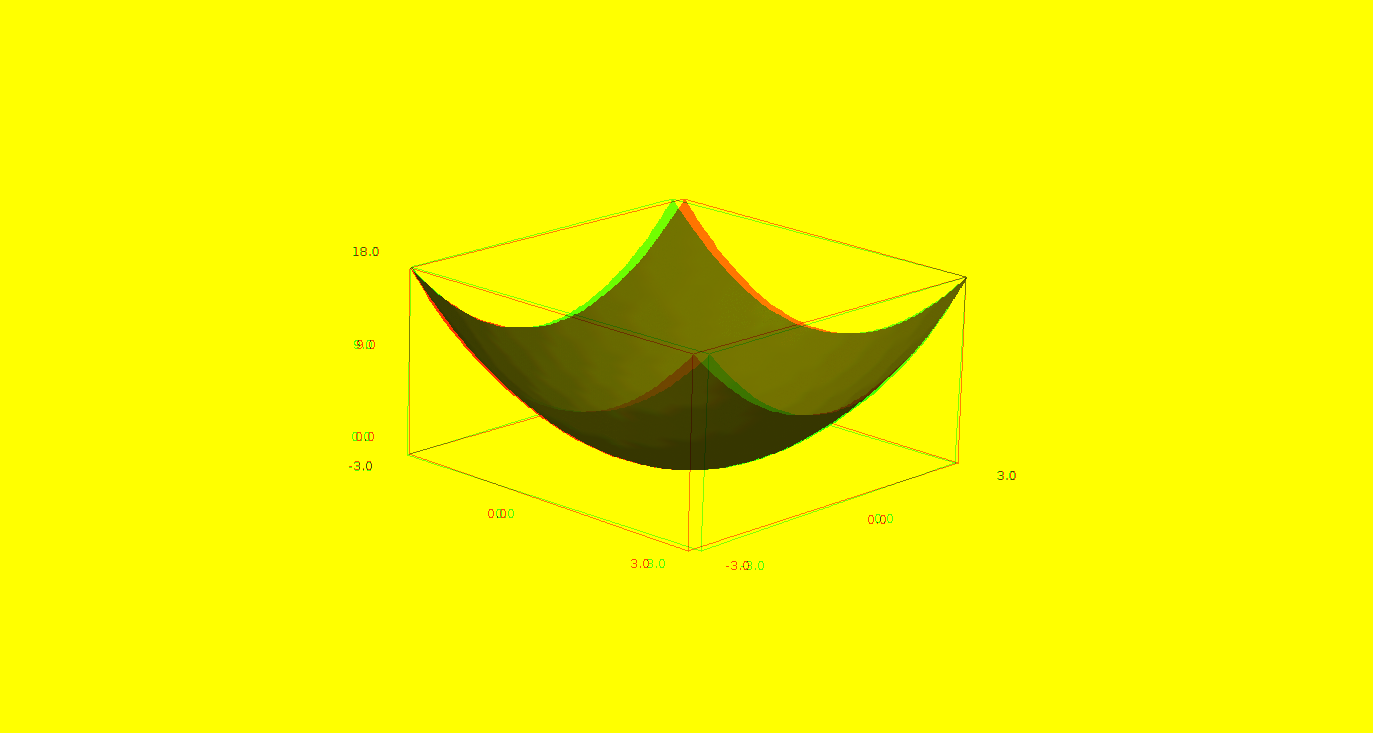
\includegraphics[width=15cm]{pictures_bitmap/coupe.png}
    \end{center}
    À part que l'ordinateur l'a dit, est-ce qu'on peut comprendre pourquoi le graphe de la fonction $x^2+y^2$ ressemble à un bol ? En coordonnées cylindriques, le graphe s'écrit
    \begin{equation}
        z=r^2.
    \end{equation}
    Donc il se fait que plus on s'éloigne du point $(0,0)$ dans le plan $XY$, plus le graphe va monter. Et il monte à quelle vitesse ? Il monte à la vitesse $r^2$. Il s'agit donc de dessiner la fonction $z=r^2$ dans le plan et de la «faire tourner».

\end{example}
